%
%
%

\begin{frame}[t,allowframebreaks]{Convolutional Network precursors: Neocognitron -}

    In 1980, \index{Fukushima}\gls{Fukushima} 
    \cite{Fukushima:1980nc, Fukushima:1988nc, Fukushima:2019nc}, 
    inspired by the studies of the \index{primary visual cortex}\gls{primary visual cortex},
    created the \index{neocognitron}\gls{neocognitron}
    as a model of the visual system.\\
    \vspace{0.2cm}

    The \gls{neocognitron} is the precursor of the \gls{cnn}.\\
    \vspace{0.2cm}

    It is a hierarchical network consisting of many 
    stages of \index{neuron}\gls{neuron}-like cells
    preceded by an input layer U$_0$.\\
    \vspace{0.2cm}

    Each stage is composed of a layer of 
    {\bf S-cells} and a layer of {\bf C-cells}.
    \vspace{0.2cm}

    \begin{itemize}
        \item
        {\bf S-cells} behave like 
        \index{simple cell}\glspl{simple cell} in the 
        \gls{primary visual cortex}: 
        \begin{itemize}
            \item
            {\bf Feature extracting} cells 
            (i.e. respond selectively to specific features)
        \end{itemize}
        \item
        {\bf C-cells} behave like 
        \index{complex cell}\glspl{complex cell} in the 
        \gls{primary visual cortex}:
        \begin{itemize}
            \item Pool responses of S-cells with 
            different receptive fields 
            (i.e. perform a spatial averaging of S-cells response)\\
        \end{itemize}
    \end{itemize}
    \vspace{0.2cm}

    \framebreak

    Each layer of cells is divided into 
    sub-layers (\index{cell-plane}\glspl{cell-plane}).
    whose cells:
    \begin{itemize}
        \item respond to the same feature,
        \item are arranged retinotopically (each cell has a different receptive field) 
        \item share the same input connections
    \end{itemize}
    %\vspace{0.1cm}
    The input connections to S-cells are variable and modified during training.
    \begin{itemize}
        \item The {\bf features extracted by an S-cell are learned}.
        \item These are {\bf local features in shallow stages} and 
              more {\bf global features in deeper stages}.
    \end{itemize}
    %\vspace{0.1cm}
    The output of a layer of S-cells is fed to a layer of C-cells.
    \begin{itemize}
        \item Fixed set of connections, from extractors of same feature
            but with slightly different receptive fields
        \item C-cells pool the response of S-cells (spatial averaging); 
        Allows robust performance for deformed patters and noise suppression.
    \end{itemize}
    %\vspace{0.1cm}
    The output of the C-cells is fed into the next layer of S-cells.\\
    %The final classification is made in the deepest stage.

    \framebreak

    \begin{center}
        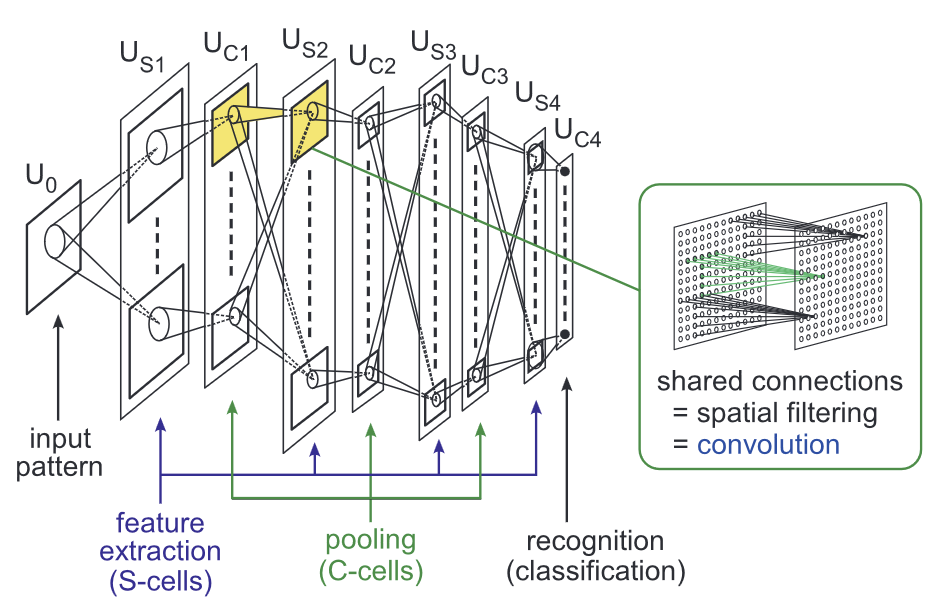
\includegraphics[width=0.80\textwidth]
           {./images/neocognitron/fukushima19_hierarchical_network_structure_01.png}\\
        {\scriptsize 
        Hierarchical network structure of the \gls{neocognitron}.\\
        $U_{S\ell}$($U_{C\ell}$) denotes the $\ell^th$ stage of S-cells (C-cells).
        $U_0$ is the input layer.\\
        \color{col:attribution} 
        Image reproduced from \cite{Fukushima:2019nc} (Fig.1)}\\
    \end{center}

    \framebreak

    \begin{columns}
        \begin{column}{0.55\textwidth}
            \begin{center}
                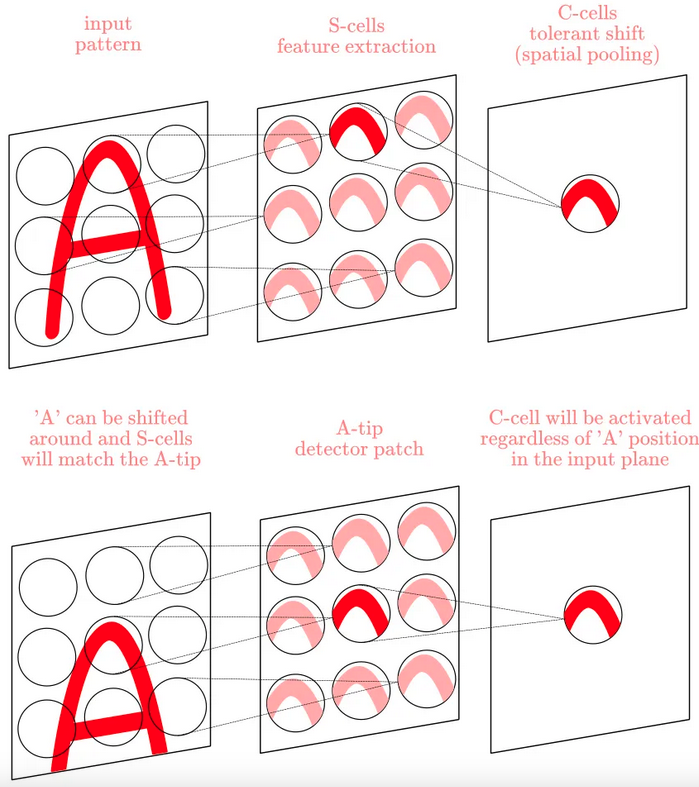
\includegraphics[width=0.90\textwidth]
                   {./images/neocognitron/elhamraoui20_feature_detection_schematic.png}\\
                {\scriptsize 
                \color{col:attribution} 
                Image reproduced from \cite{Medium:LeNet5andAlexNet}}\\
            \end{center}
        \end{column}
        \begin{column}{0.45\textwidth}
            \begin{center}
                Position-independence of feature detection in the \gls{neocognitron}.\\
            \end{center}
        \end{column}
    \end{columns}

\end{frame}


